\section{Algorithmes de programmation}
\label{sec:algor-de-progr}

\subsection{Organigramme du Pong}
\label{sec:organigramme}

\begin{figure}[!h]
  \centering
  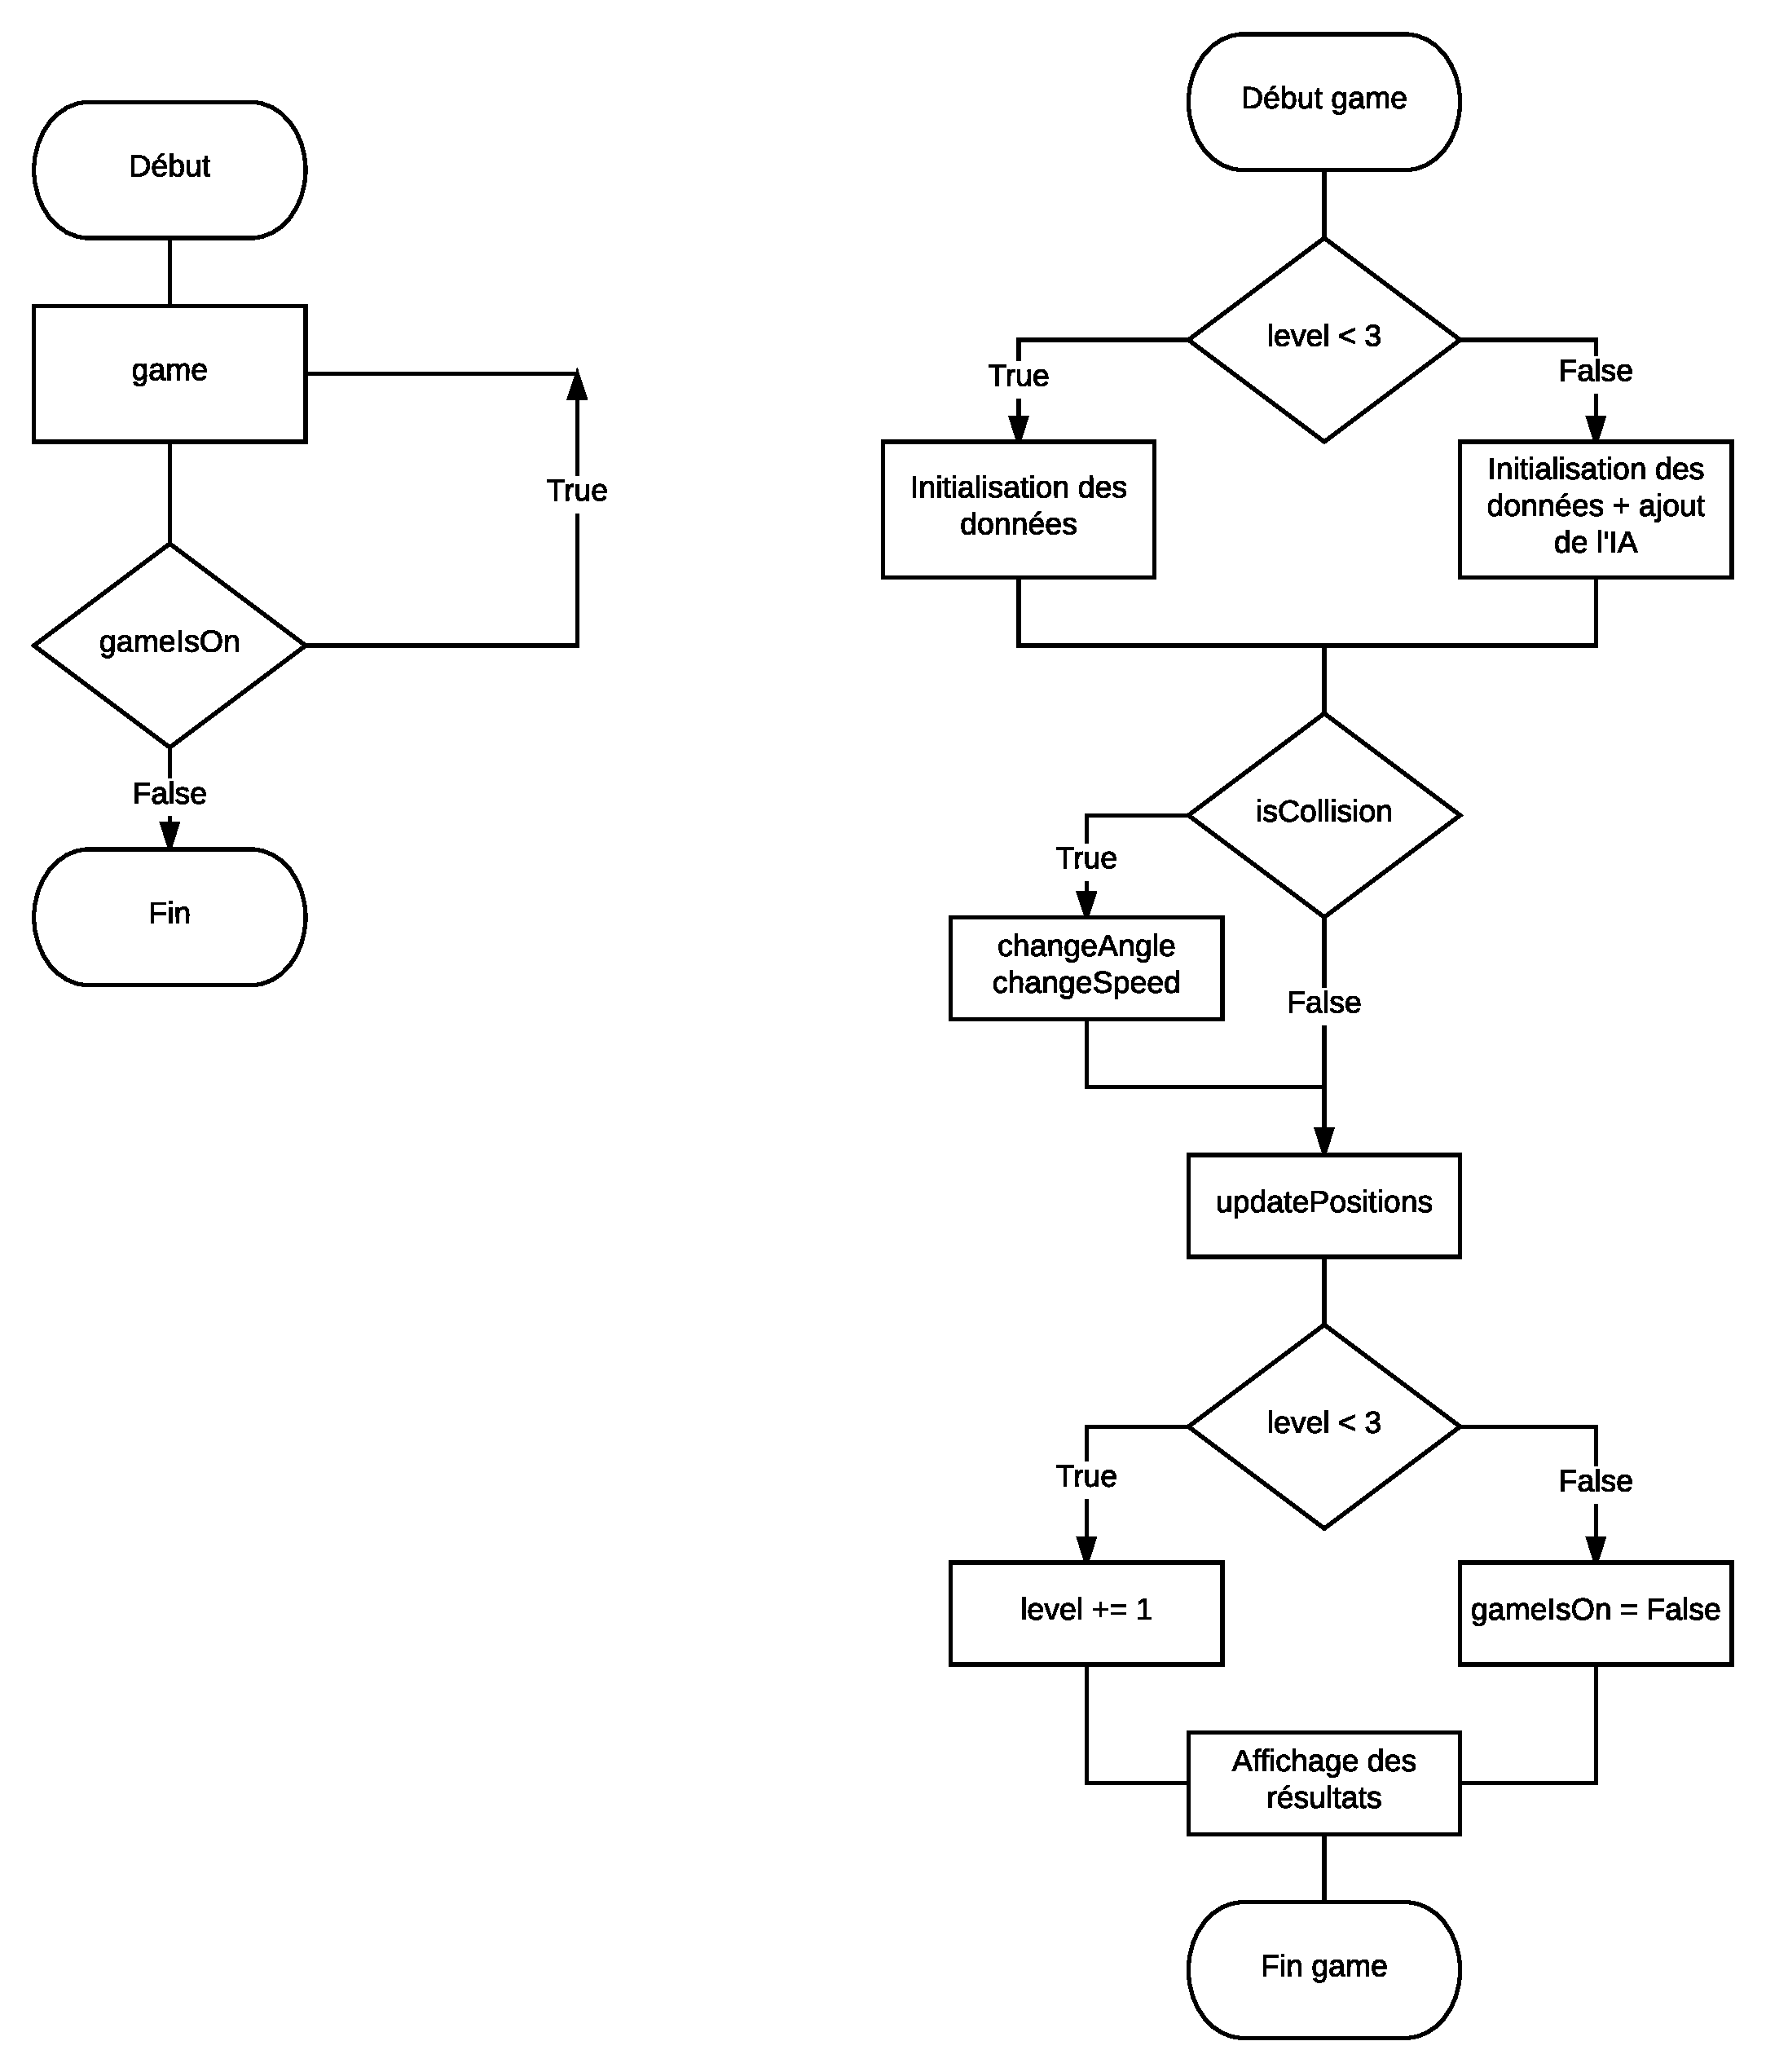
\includegraphics[scale=0.4]
  {textures/images/algorithm/organigram.pdf}
  \caption{Organigramme du PyPong}
  \label{fig:organigram}
\end{figure}

\newpage

\subsection{Collisions en détails}
\label{sec:collisions-details}

Dans ce point, il sera question de détailler le code de détection des différentes
collisions du Pong. Liée à cela, la gestion des angles sera aussi explicitée.

Pour débuter, nous avons choisi - \textit{au début du projet} - de définir le
référentiel d'après la balle. Pour elle, l'axe des abscisses est l'axe sur lequel
les raquettes se déplacent.

\subsubsection{Collision avec les murs}
\label{sec:collision-murs}

\begin{minted}{Python}
def isWallCollision(self):
    if self.level < 3:
        if self.ball.x == 0 or self.ball.x == self.row - 1:
            #Roof
            self.ball.dx = -self.ball.dx
            self.result += 3
            self.ball.speed -= 0.1
        if self.ball.y == 0:
            #Left side
            self.ball.dy = -self.ball.dy
            self.result += 3
            self.ball.speed -= 0.1
    else:
        if self.ball.x == 0 or self.ball.x == self.row - 1:
            #Roof
            self.ball.dx = -self.ball.dx
            self.ball.speed -= 0.1
\end{minted}

Dans ce cas, deux cas sont possibles: soit on est dans un des deux premiers
niveaux et on joue seul contre le mur de gauche, soit on joue contre
l'intelligence artificielle.

\begin{itemize}

    \item Prenons le premier cas, la balle peut donc rebondir sur trois surfaces: celle du
    haut, celle du bas et celle de la gauche.

    \item Prenons le second cas où la balle ne peut rebondir que sur les bords
    supérieurs et inférieurs.

\end{itemize}

La collision avec le haut ou le bas se fait respectivement quand la position
\textbf{x} est soit nulle, soit la dernière position possible dans les limites
de la grille.\\
La collision avec le mur gauche se fait de manière similaire, mais seulement
lorsque la position \textbf{y} est nulle que la balle entre en collision avec le
mur. \\

Lors d'une collision, la vitesse et le résultat sont augmentés, et la direction
\textbf{x} ou \textbf{y} est inversée. \\
Dans le cas où la balle va dans un coin gauche, elle subit les deux collisions:
le joueur gagne le double de points et la vitesse est encore plus rapide.

\newpage

\subsubsection{Collision avec les raquettes}
\label{sec:collision-raquettes}

\begin{minted}{Python}
def isPaddleCollision(self):
    if self.level < 3:
        if self.ball.y == self.column - 2 and
        self.ball.x == self.paddle.x:
            self.ball.dy = -self.ball.dy
            self.result += 2
            self.ball.speed -= 0.15
    else:
        if (self.ball.y == 1 and
        self.ball.x == self.paddleLeft.x) or
        (self.ball.y == self.column - 2 and
        self.ball.x == self.paddleRight.x):
            self.ball.dy = -self.ball.dy
            self.ball.speed -= 0.15
\end{minted}

Deux cas sont à nouveaux possibles: si le joueur se retouve contre
l'intelligence artificielle, alors il y a deux raquettes en jeu. Sinon, la balle
ne peut rebondir que sur la raquette de droite.

\begin{itemize}

    \item Dans le cas sans l'intelligence artificielle, il suffit que la balle
    soit aux coordonnées de la raquette pour qu'il y ait une collision. \\
    Lors de la collision, le résultat est augmenté de 2.

    \item Dans l'autre cas, la condition change légèrement: la balle doit
    toujours se trouver dans la colonne de la raquette \textit{(la deuxième à
    gauche ou l'avant-dernière à droite)}, et à la ligne de la bonne raquette
    \textit{(respectivement la gauche ou la droite)}.

\end{itemize}

S'il y a une collision avec une raquette, seule la direction \textbf{y} est
inversée dans le but de garder des angles à 45$^{\circ}$, et l'accélération est
légèrement supérieure à celle observée lors de la collision avec un mur.

\newpage

\subsubsection{Sortie des limites}
\label{sec:sorties-limites}

\begin{minted}{Python}
def isOut(self):
    if self.level < 3:
        return self.ball.y == self.column - 1
    return self.ball.y == 0 or self.ball.y == self.column - 1
\end{minted}

Cette méthode est très simple. \\
Comme pour les autres collisions, il y aura le cas du niveau 3, et celui des
niveaux inférieurs.

\begin{itemize}

    \item Pour le niveau 3, la balle sort de la grille de jeu si elle touche
    le bord gauche ou le bord droit \textit{(soit la première colonne, soit
    la dernière)}.

    \item Pour les autres niveaux, la balle pouvant, \textit{(devant)}, rebondir
    sur le bord de gauche, seule une collision sur le bord droit est vue comme
    une sortie hors de la grille.

\end{itemize}

%%% Local Variables:
%%% mode: latex
%%% TeX-master: t
%%% End:
